\section{FLWOR Expressions}
\label{sect:trans:TD:simpleFLWOR}
The \texttt{let} clause does not explicitly cause any dependencies, only variable binding, and can therefore be
translated into storing the algebraic version of the expression to be bound in
the symbol table (see section \ref{sect:trans:TD:basics}):
\begin{equation}
\frac{}{\mbox{\texttt{let \$}}\chi \mbox{\texttt{ := }}e \mbox{\texttt{ \ldots}}}\longmapsto
\mbox{\textbf{put(}}\chi\mbox{\textbf{, r(}}e\mbox{\textbf{))}}
\label{rule:trans:TD:letbind}
\end{equation}
The iterator dependences $e.\vartheta$ is stored along with \textbf{r(}$e$\textbf{)} and will piggyback this
algebra tree if it later fetched from the symbol table. If there is more than one variable binding in the
\texttt{let} clause the rule must be applied once per binding as if one binding were one \texttt{let} clause.

As seen by the excerpt of the W3C XQuery EBNF specification in figure
\ref{fig:trans:TD:seqEBNF}, a FLWOR expression may be structured in many
different ways. For simplicity and readablilty the translation of such
expressions will be split up in more managable pieces.

A FLWOR expression may have multiple \texttt{for}-clauses, and a \texttt{for}-clause may have multiple iterator
variable bindings. This means that one FLWOR may consist of many iterators, the semantics of which is described in
section \ref{sect:method:ast_rewrite}. We assume all possible iterator dependencies generated from the FLWOR, that
is, all iterator variables bound, is stored in a ordered set $\beta$. The dependencies are ordered in the order of
which the corresponding iterator variables are bound, i.e. top down, left to right while parsing the query. When
enclosed in MQL syntax $\beta$ is, as $\vartheta$, to be read as a comma separated list of the attributes
corresponding to the dependencies.

\begin{figure}[h]
\centering
\begin{tabular}{l}
$[$\texttt{for}/\texttt{let \ldots}$]+$ \\ \quad
$[$\texttt{where }$e_2]?$ \\ \quad
$[$\texttt{order by }$e_3]?$ \\
\texttt{return }$e_4$
\end{tabular}
\label{fig:trans:TD:flworIll}
\caption{Illustration of a FLWOR expression}
\end{figure}

The translation of a single FLWOR like the one illustrated in figure \ref{fig:trans:TD:flworIll} will be executed
as shown in figure \ref{fig:trans:TD:flworExecute}. Firstly, all \texttt{for} and \texttt{let} variables will be
bound as described by the rules \ref{rule:trans:TD:forbind} and \ref{rule:trans:TD:letbind}, respectively.
Further, the \texttt{return}-clause will be evaluated. If there is a \texttt{where}-clause present, it is
evaluated next, based on the \texttt{where}-expression and the result of the \texttt{return}-clause, referred to
as \textbf{r(}$e_{C}$\textbf{)}. The order of the items returned from the FLWOR is conditioned by the presence of
an \texttt{order by}-clause in the expression. If there is a \texttt{order by}-clause, it will order the
intermediate result from the \texttt{return} or \texttt{while}-clause, and finalise the FLWOR. If there is no
\texttt{order by}-clause, the final evaluation of the FLWOR will be to order the intermediate result according to
the iterators.

\begin{figure}[h]
\centering

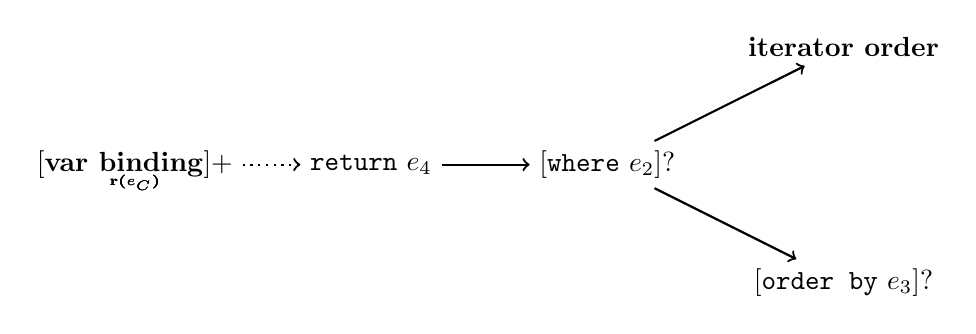
\begin{tikzpicture}

\node (bind) at (0,0) {$[$\textbf{var binding}$]+$};
\node (return) at (3,0) {\texttt{return} $e_{4}$};
\node (where) at (6,0) {$[$\texttt{where} $e_{2}]?$};
\node (itord) at (9,1.5) {\textbf{iterator order}};
\node (ordby) at (9,-1.5) {$[$\texttt{order by} $e_{3}]?$};
\draw [->,dotted,thick] (bind) to (return);
\draw [->,thick] (return) to (where) node[below,midway] {\tiny\textbf{r(}$e_{C}$\textbf{)}};
\draw [->,thick] (where) to (itord) node[below,midway] {\tiny\textbf{r(}$e_{C}$\textbf{)}};
\draw [->,thick] (where) to (ordby) node[below,midway] {\tiny\textbf{r(}$e_{C}$\textbf{)}};
\end{tikzpicture}
\label{fig:trans:TD:flworExecute}
\caption[FLWOR translation order]{Illustration of step-by-step translation of FLWOR.}
\end{figure}



Any possible iteration, ordering og filtering will be handled by other clauses than the \texttt{return}-clause.
The \texttt{return}-clause will just ship the evaluated version of the \texttt{return}-expression forward:
\begin{equation}
\frac{}{\mbox{\texttt{return }}e_{4}}\longmapsto
\mbox{\textbf{r(}}e_{4}\mbox{\textbf{)}}
\label{rule:trans:TD:returnTaint}
\end{equation}


\subsection{Iterator Ordering}
Acording to XQuery semantics, the \texttt{return} clause is evaluated once for iteration for each of the iterators
of the FLWOR expression. The results of these evaluations are concatenated to form the result of the FLWOR
expression. As TD evaluate iterations in parallel, if the \texttt{return}-expression is not dependent on a
iterator, its relational form will not have a representation for each of the iterators iterations and will have to be tainted.

Because each FLWOR iterator creates a new sequence, renumbering is needed. No expression in a sibling or parent
scope of the FLWOR may be dependent on the dependencies in $\beta$. Thus, $\beta$ is not part of the dependencies
returned from the FLWOR, and the attributes corresponding to $\beta$ must be removed. 

If the FLWOR contains no \texttt{order by}-clause, the ordering of the resulting sequence is determined by the
iterators of the expression. Remember, the set of iterators $\beta$ is ordered according to the order the
variables were bound.
\begin{equation}
\frac{}{\mbox{\textbf{iterator order}}}
\longmapsto
\begin{array}{l}
\mbox{\textsf{numberate(index, [}}\beta\mbox{\textsf{, index], [}}\vartheta\mbox{\textsf{];}} \\ \quad
\mbox{\textbf{t(r(}}e_{C}\mbox{\textbf{), }}\beta\mbox{\textbf{)}}
\end{array}
\label{rule:trans:TD:itOrd}
\end{equation}

Where $\vartheta = e_{C}.\vartheta - \beta$, and $e_C$ is the result returned from the \texttt{where}-clause, if
present, otherwise it is the result of the \texttt{return}-clause.

From equation \ref{eq:trans:TD:taint} it is clear that an expression already dependent on any iterator in $\beta$
will not be tainted by these iterators.

The \textsf{numberate} operator will have to partition on the remaining dependencies in $\vartheta$ to seperate
the sequences returned from the iterator for all iterators the result is dependent on, as described in section
\ref{sect:trans:TD:implic}.

\begin{myExample}
Consider the query of figure \ref{fig:trans:TD:dblFor}. Notice the expression in the \texttt{return} clause ($e_1$)
is the same as $e_1$ in example \ref{ex:trans:TD:simpleSeq}.

\begin{figure}[h]
\begin{equation*}
\begin{array}{l}
\mbox{\texttt{for \$a in (10,20),}} \\
\mbox{\texttt{\phantom{abcd}\$b in (50,75)}} \\ 
\mbox{\texttt{return }}\underbrace{\mbox{\texttt{(\$a, "no")}} }_{e_{1}}
\end{array}
\end{equation*}
\caption{Example query with two iterators.}
\label{fig:trans:TD:dblFor}
\end{figure}

Expression $e_{1}$ is not depentant on $I_{\mbox{\texttt{b}}}$, and by rule \ref{rule:trans:TD:itOrd} will be
tainted by this iterator. The result of the tainting is shown in figure \ref{fig:trans:TD:final:taint}. The
expression will however not be tainted by $I_{\mbox{\texttt{a}}}$, as it is already dependent on this iterator
(ref. equation \ref{eq:trans:TD:taint}).

\begin{figure}[h]
\centering
\subfigure[\textbf{t(r(}$e_{1}$\textbf{), \{}\texttt{b}\textbf{\})}]{
\begin{tabular}{|c|c|c|c|} \hline
$bnb$ & $anb$ & $idx$ & $val$ \\ \hline
1 & 1 & 1 & 10 \\ \hline
1 & 2 & 1 & 20 \\ \hline
1 & 1 & 2 & \texttt{"no"} \\ \hline
1 & 2 & 2 & \texttt{"no"} \\ \hline
2 & 1 & 1 & 10 \\ \hline
2 & 2 & 1 & 20 \\ \hline
2 & 1 & 2 & \texttt{"no"} \\ \hline
2 & 2 & 2 & \texttt{"no"} \\ \hline
\end{tabular}
\label{fig:trans:TD:final:taint}
}
\qquad
\subfigure[\textbf{r(}$I_{\mbox{\texttt{a}}}$\textbf{)}]{
\begin{tabular}{|c|c|} \hline
$idx$ & $val$ \\ \hline
1 & 10 \\ \hline
2 & \texttt{"no"} \\ \hline
3 & 10 \\ \hline
4 & \texttt{"no"} \\ \hline
5 & 20 \\ \hline
6 & \texttt{"no"} \\ \hline
7 & 20 \\ \hline
8 & \texttt{"no"} \\ \hline
\end{tabular}
\label{fig:trans:TD:final:rIa}
}
\caption[Example: resolving simple FLWOR]{Evaluating the query in figure \ref{fig:trans:TD:dblFor} yields the
intermediate result (a) and the final result (b). Attribute names are
shortened.
\label{fig:trans:TD:finaliseExp}}
\end{figure}

With the expression tainted the dependencies of all the iterators of the FLWOR, renumbering is the last operation
required to translate the query. The \textsf{numberate} operator will sort the tuples first on $anumb$, then on
$bnumb$ and finally $index$ before numbering. As the FLWOR itself does not have any dependencies the numeration
will not be partitioned over any attributes. The result of the query is shown in figure
\ref{fig:trans:TD:final:rIa}.
\end{myExample}

\subsection{Where-Clause}
The W3C describes the FLWOR expression as generating a tuple stream which contains one tuple for each combination
of values bound in the expression\cite{w3c00}. In this view, the optional \texttt{where}-clause serves a filter
for these tuples. The expression in the \texttt{where}-clause is evaluated once for each tuple. If the boolean
value of this expression is $true$, the tuple is retained, if the boolean value is $false$ the tuple is discarded.

The \texttt{where}-clause can be evaluated by only selecting the iteration combinations where the
\texttt{where}-expression is $true$. The result of this will be joined with the result of the \texttt{return}
clause. If the result from the \texttt{return}-clause and the \texttt{where}-expression has no common iterator
dependencies, the equi-join will have to be replaced by a cartesian product, as discussed in
\ref{sect:trans:TD:implic}.

\begin{equation}
\frac{}{\mbox{\texttt{where }}e_2}\longmapsto
\begin{array}{l}
\mbox{\textsf{hhjoin([}}(e_{C}.\vartheta \cap e_2.\vartheta)\mbox{\textsf{], [}}(e_{2}.\vartheta \cap
e_{C}.\vartheta)\mbox{\textsf{], [l.value, }} \vartheta\mbox{\textsf{];}} \\ \quad
\mbox{\textbf{r(}}e_{C}\mbox{\textbf{)\textsf{;}}} \\ \quad
\mbox{\textsf{select(xqBoolean(pred);}} \\ \quad \quad
\mbox{\textbf{B(r(}}e_{2}\mbox{\textbf{)}\textsf{)))}}
\end{array}
\label{rule:trans:TD:where}
\end{equation}

Where $\vartheta = e_{C}.\vartheta \cup e_{2}.\vartheta$, and \textbf{r(}$e_{C}$\textbf{)} is the result of the
translation done in the \texttt{return}-clause.

By employing the \textsf{select} operator before the joining of the two relations the number of tuples needed
involved in the join will be minimised. Further, as the \textsf{hhjoin} operator allows for declaring which
attributes to be projected, there is no need for a seperate \textsf{project} operator.

\begin{myExample}
Consider the XQuery query of figure \ref{fig:trans:TD:whereQuery}. The evaluation of $e_{1}$ is very similar to
the evaluation of $e_{1}$ of example \ref{ex:trans:TD:simpleSeq}, and the
result is shown in figure \ref{fig:trans:TD:where:re1}. The \texttt{where}-clause contains a comparison
expression, which will be discussed later. Figure \ref{fig:trans:TD:where:whereE} shows the result relation of the
\texttt{where}-expression.

\begin{figure}[h]
\centering
\begin{equation*}
\begin{array}{l}
\mbox{\texttt{for \$a in (10,20)}} \\
\mbox{\texttt{where \$a > 15}} \\
\mbox{\texttt{return}} \underbrace{\mbox{\texttt{(\$a, 14)}}}_{e_{1}}
\end{array}
\end{equation*}
\caption{A FLWOR expression with a \texttt{where}-clause \label{fig:trans:TD:whereQuery}}
\end{figure}

\begin{figure}[h]
\centering
\subfigure[\textbf{r(}$e_{1}$\textbf{)}]{
\begin{tabular}{|c|c|c|} \hline
$anb$ & $idx$ & $val$ \\ \hline
1 & 1 & 10 \\ \hline
1 & 2 & 14  \\ \hline
2 & 1 & 20 \\ \hline
2 & 2 & 14  \\ \hline
\end{tabular}
\label{fig:trans:TD:where:re1}
}
\qquad
\subfigure[\textbf{r(}\texttt{\$a > 15}\textbf{)}]{
\begin{tabular}{|c|c|c|} \hline
$anb$ & $idx$ & $val$ \\ \hline
1 & 1 & $false$ \\ \hline
2 & 1 & $true$ \\ \hline
\end{tabular}
\label{fig:trans:TD:where:whereE}
}
\qquad
\subfigure[]{
\begin{tabular}{|c|c|c|} \hline
$anb$ & $idx$ & $val$ \\ \hline
2 & 1 & 20 \\ \hline
2 & 2 & 14  \\ \hline
\end{tabular}
\label{fig:trans:TD:where:intr}
}

\caption[Example: Evaluation of where clause]{Applying rule \ref{rule:trans:TD:where} on (a) and (b)
yields (c). Attribute names are shortened. \label{fig:trans:TD:whereClause}}
\end{figure}

During the evaluation of the FLWOR, the tuples in the \texttt{where}-expression relation where $value$ ($val$ in
figure) is not $true$ will be removed. The result is a relation with a single tuple where $anumb$ holds the value
$2$. This result is then joined with the $e_1$ relation on $anumb$, as shown in figure
\ref{fig:trans:TD:where:intr}. Rule \ref{rule:trans:TD:itOrd} will have to be applied to complete the
evaluation of the query.
\end{myExample}


\subsection{Order By-Clause Ordering}

As can be seen in figure \ref{fig:trans:TD:ordEBNF}, an \texttt{Order by}-clause may contain several
specifications on how to order and what to order by.
\begin{figure}[h]
\begin{Verbatim}
[38] OrderByClause ::= (("order" "by") | ("stable" "order" "by")) 
                           OrderSpecList
[39] OrderSpecList ::= OrderSpec ("," OrderSpec)*
[40] OrderSpec     ::= ExprSingle OrderModifier
[41] OrderModifier ::= ("ascending" | "descending")? 
                           ("empty" ("greatest" | "least"))? 
                           ("collation" URILiteral)?
\end{Verbatim}
\label{fig:trans:TD:ordEBNF}
\caption[W3C EBNF order by clause specification]{W3C EBNF order by clause specification\cite{w3c00}.}
\end{figure}

At this time, Taiting Dependencies only support a simple form of the clause. Only one \texttt{OrderSpec} is
allowed, where the expression to be sorted on will be referred to as $e_4$ -- conformant to figure
\ref{fig:trans:TD:flworExecute}. Nor is any \texttt{OrderModifier}s allowed. A complete translation of the
\texttt{order by}-clause is discussed in section \ref{sect:disc:orderby}.

As with the \texttt{where}-clause W3C specify the \texttt{order by}-clause as operating on a tuple stream created
by the variable bindings in the FLWOR\cite{w3c00}. The clause causes the stream to be reordered into a new,
value-based order. This means that the iterator dependency attributes ($\chi{numb}$) will no longer decide the
composition of the sequence returned from the FLWOR.

Firstly, to ensure that the result will have a representation for all the iterations (still valid after possible
filtering by \texttt{where}-clause) of all the expressions iterators, $e_C$ is tainted with $\beta$. The
\texttt{order by}-expression is evaluated and joined with the result of the tainting on their common iterator
dependencies. Lastly, this relation is renumbered according to the order of the values stemming from the
\texttt{order by}-expression:

\begin{equation}
\frac{}{\mbox{\texttt{order by }}e_3}\longmapsto
\begin{array}{l}
\mbox{\textsf{project(value = l.value, }}\vartheta\mbox{\textsf{;}}\\ \quad
\mbox{\textsf{numberate(index, [r.value], [}}\vartheta\mbox{\textsf{];}} \\ \quad \quad
\mbox{\textsf{hhjoin([}}(e_{C}.\vartheta \cap e_2.\vartheta)\mbox{\textsf{], [}}(e_{2}.\vartheta \cap
e_{C}.\vartheta)\mbox{\textsf{],}} 
\mbox{\textsf{[l.value, r.value, }} \vartheta\mbox{\textsf{];}} \\ \quad \quad
\quad \mbox{\textbf{t(r(}}e_C\mbox{\textbf{), }}\beta\mbox{\textbf{)}\textsf{;}} \\ \quad \quad \quad
\mbox{\textbf{r(}}e_3\mbox{\textbf{)}\textsf{)))}}
\end{array}
\label{rule:trans:TD:orderbyOrd}
\end{equation}

Where $\vartheta = (e_C.\vartheta \cup e_3.\vartheta)-\beta$, and \textbf{r(}$e_{C}$\textbf{)} is the result of
the translation done in the \texttt{where}-clause if present, else the
\texttt{return}-clause. Fields such as $index$ and if applicable $documentId$, $pos$ and $scope$ will follow
$l.value$. $r.value$ is only the $value$ column from the right relation. To accommodate for the \texttt{stable}
keyword, the \textsf{numberate} operator will have to sort on $l.index$ aswell, after sorting on $r.value$.

As desired, all iterator dependency attributes ($\chi{numb}, \chi \in \beta$) will be projected away by the
\textsf{hhjoin} operator. An additional \textsf{project} operator is used to ensure that the $value$ returned from
the expression is the $value$ attribute of the \texttt{return}-expression.

\begin{myExample}
Figure \ref{fig:trans:TD:ordQu} shows a query consisting of a FLWOR expression containing a \texttt{order by} clause.
\begin{figure}[h]
\centering
\begin{tabular}{l}
\texttt{for \$a in (4, 6, 8)} \\
\texttt{order by \$a mod 3}\\
\texttt{return \$a}\\
\end{tabular}
\label{fig:trans:TD:ordQu}
\caption{Example query with order by clause}
\end{figure}

The evaluated \texttt{order by}-expression is shown in figure \ref{fig:trans:TD:ord:oExp}. How modulus expressions
are translated will be discussed later. After their evaluation, the relational representation of \texttt{order
by}-expression relation and the \texttt{return}-clause is joined on their common iterator dependencies,
$I_{\mbox{\texttt{a}}}$ ($anumb$). The result of the join is shown in figure \ref{fig:trans:TD:ord:join}. Lastly,
this relation is renumbered and sorted on the $r.value$ ($r.val$ in figure) attribute stemming from the
\texttt{order by}-expression, as shown in figure \ref{fig:trans:TD:ord:numb}. An additional projection to rename
$l.value$ to $value$ is needed to finalise the query.

\begin{figure}[h]
\centering
\subfigure[\textbf{r(}\texttt{\$a mod 3}\textbf{)}]{
\begin{tabular}{|c|c|c|} \hline
$idx$ & $anb$ & $val$ \\ \hline
1 & 1 & 1 \\ \hline
1 & 2 & 0 \\ \hline
1 & 3 & 2 \\ \hline
\end{tabular}
\label{fig:trans:TD:ord:oExp}
}
\qquad
\subfigure[]{
\begin{tabular}{|c|c|c|c|} \hline
$l.idx$ & $anb$ & $l.val$ & $r.val$ \\ \hline
1 & 1 & 4 & 1 \\ \hline
1 & 2 & 6 & 0 \\ \hline
1 & 3 & 8 & 2 \\ \hline
\end{tabular}
\label{fig:trans:TD:ord:join}
}
\qquad
\subfigure[]{
\begin{tabular}{|c|c|} \hline
$idx$ & $l.val$ \\ \hline
1 & 6 \\ \hline
2 & 4 \\ \hline
3 & 8 \\ \hline
\end{tabular}
\label{fig:trans:TD:ord:numb}
}


\caption{Intermediate results evaluating the query of figure
\ref{fig:trans:TD:ordQu}. (a) shows the evaluated \texttt{order by} expression. (b) shows the \texttt{order
by}-expression joined with the \texttt{return}-expression. (c) shows the relation in (b) renumbered. Attribute
names are shortened.\label{fig:trans:TD:orderRes}}
\end{figure}


\end{myExample}
